% !TEX root = ../../main.tex
\subsection*{Publication-scale GTR simulations and multiple-testing controls}

We repeated the corrected head-to-head experiment on the publication grid (1,000
replicates per cell; 100, 250, and 1,000 sites; branch lengths 4--12; five-taxon
external and 16-taxon internal targets) using the fixed GTR+F, GTR+F+G4 and
GTR+F+I+G4 specifications.  Each replicate records the dominant and
eigenvalue-weighted statistics, branch-level audit, decision-rule audit, and
timing information.  The merged GTR grid contains 864,000 detail rows and
2,016 summary rows, with 1,000 replicates in every evaluated cell; the native
calculation invariant has zero JC-collapse mismatches.

Under the unadjusted rule, the largest paired increase in the informative-call
fraction was 0.241 (95\% bootstrap interval 0.215--0.269; exact McNemar
$p=5.7\times10^{-73}$) for GTR+F+G4 at 100 sites and branch length 12 on the
16-taxon target in the true-topology/ML-length scenario.  With taxon-level
Bonferroni correction the largest increase was 0.576 (95\% interval
0.546--0.607; $p=8.1\times10^{-174}$), and with the Benjamini--Yekutieli rule
it was 0.414 (95\% interval 0.384--0.446; $p=4.7\times10^{-125}$).  These are
paired replicate comparisons, so the intervals and tests quantify the change
in calls rather than treating the two formulas as independent samples.

The independent dominant, eigenvalue-weighted, and paired-difference plots are
shown for the matched GTR case in Fig.~\ref{fig-gtr-matched-2d}; the fixed
GTR+G4 and GTR+I+G4 paired curves are included in the supplementary figure
set.  The corresponding vector 3D views preserve the site, branch-length, and
tree-case dimensions without rasterising the surface (supplementary figures).

We then evaluated the same simulated GTR+F alignments under JC, K2P, and F81
to quantify model misspecification.  The corrected misspecification grid
contains 960,000 detail rows and 2,208 summaries, with 1,000 replicates in
every available cell.  The largest unadjusted paired increase was 0.131
(95\% interval 0.107--0.157; $p=2.4\times10^{-24}$) for GTR evaluated by K2P
at 100 sites and branch length 8 on the 16-taxon ML tree.  Under taxon
Bonferroni the largest increase was 0.206 (0.176--0.236; $p=5.3\times10^{-39}$),
and under BY it was 0.209 (0.180--0.240; $p=1.1\times10^{-38}$).  The JC,
K2P, and F81 comparisons are shown independently in the supplementary 2D and
3D figure sets.

The matched protein suite extends the same 1,000-replicate design to fixed
LG+G4, WAG+G4, JTT+G4 and Q.pfam+G4 models. Across the 1,728
model--rule--grid cells, the weighted-minus-dominant informative-call
difference was positive in 831 cells and zero in 897; it was negative in none.
The largest unadjusted increases were 0.030 for LG (95\% interval
0.020--0.041), 0.075 for WAG (0.059--0.092), 0.479 for JTT
(0.447--0.510), and 0.041 for Q.pfam (0.029--0.054). Under taxon Bonferroni,
the corresponding maxima were 0.327 (0.298--0.356), 0.469
(0.438--0.499), 0.555 (0.524--0.587), and 0.354 (0.325--0.384). Under
Benjamini--Yekutieli they were 0.094 (0.076--0.113), 0.165
(0.142--0.188), 0.514 (0.483--0.545), and 0.118 (0.099--0.138). As in the
nucleotide grid, the largest differences occurred at 100 sites and long
target branches. Figure~\ref{fig-protein-bonferroni} shows the four
model-specific taxon-Bonferroni surfaces; the unadjusted and
Benjamini--Yekutieli views and all interactive 3D panels are supplied with the
complete figure bundle.

\begin{figure}[p]
  \centering
  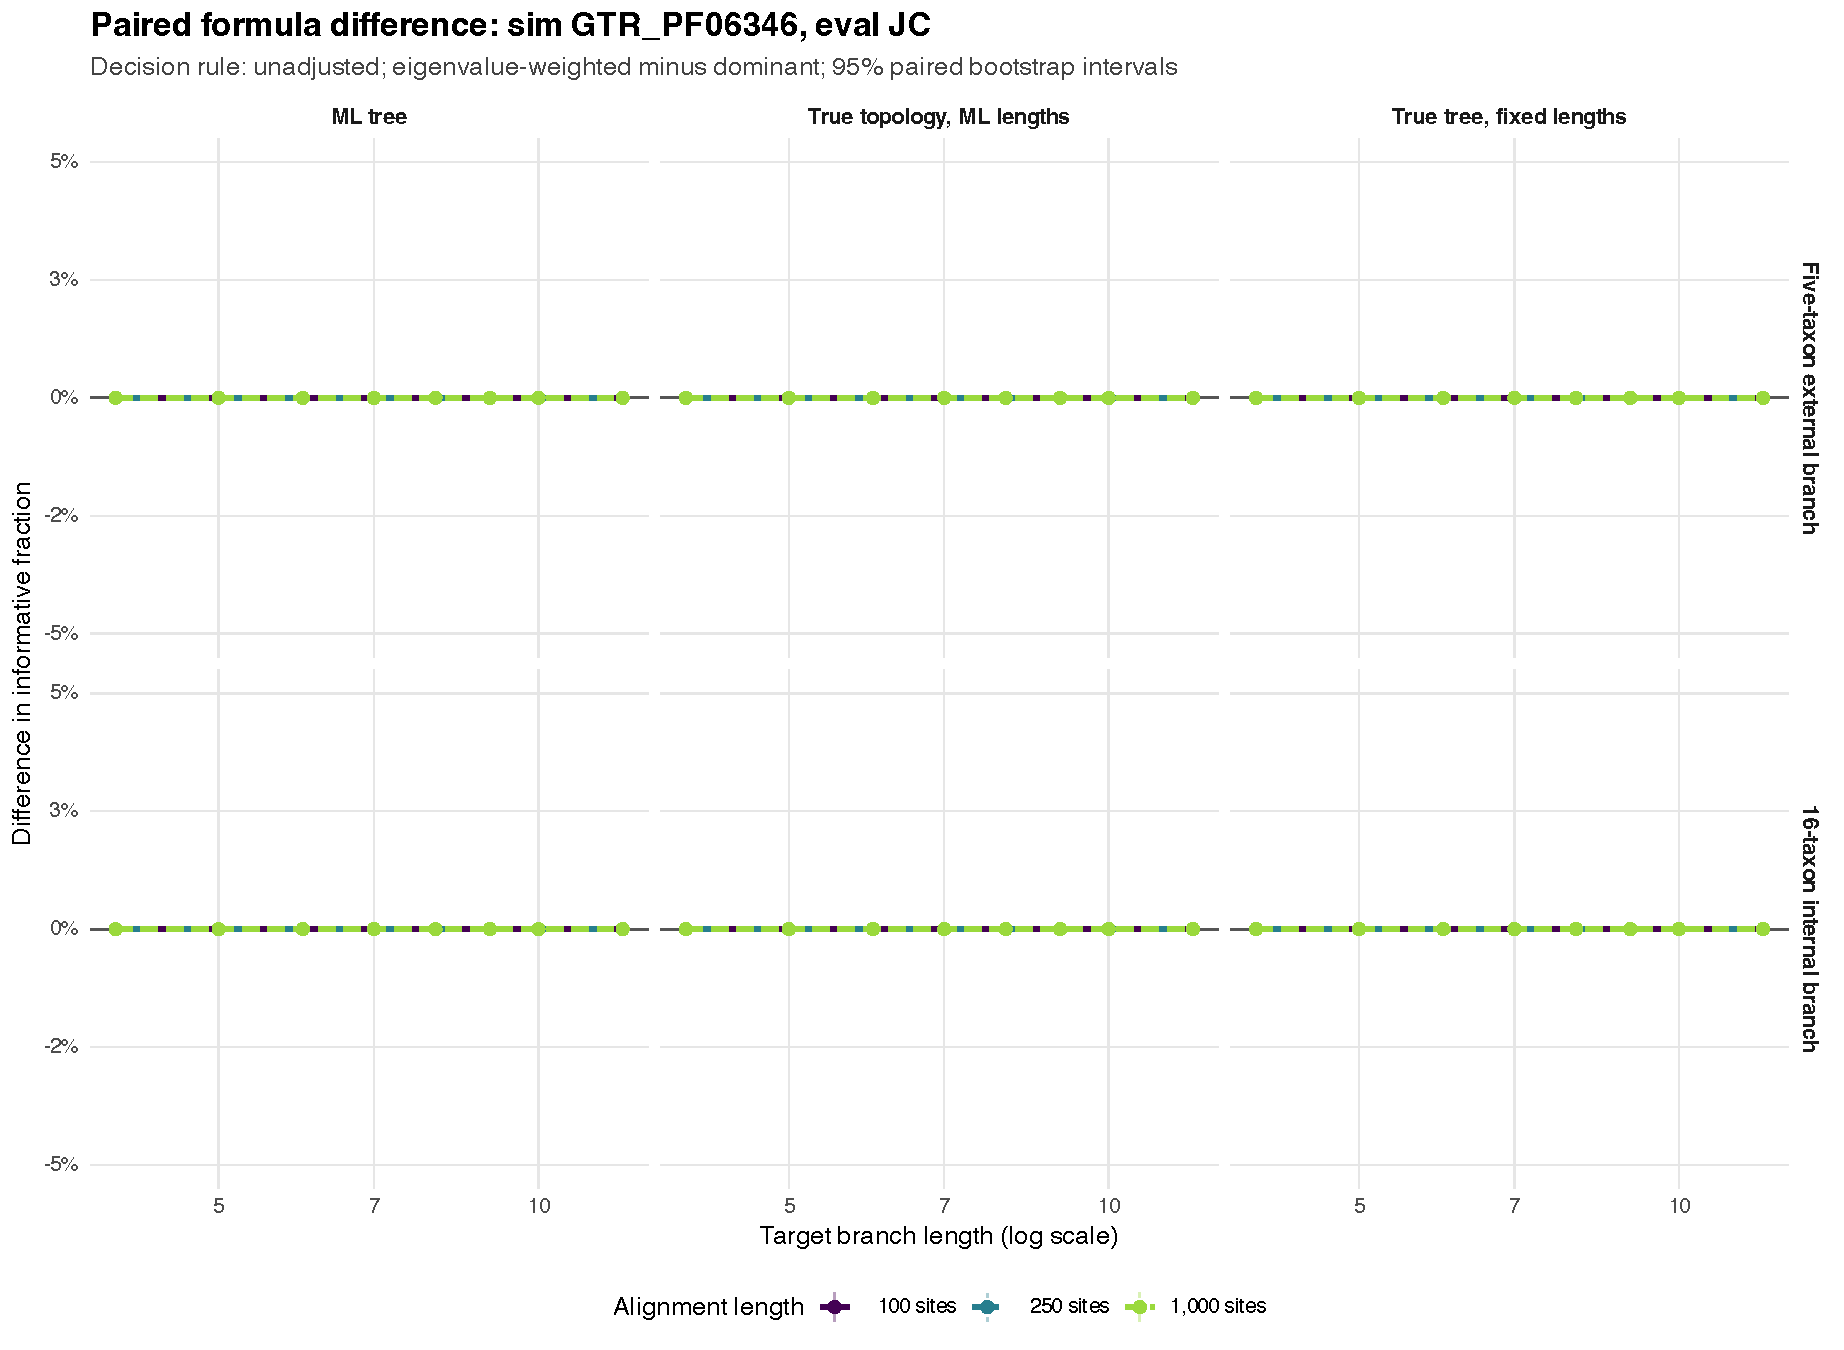
\includegraphics[width=0.32\textwidth]{figures/publication-suite/figure_gtr_misspec_JC_paired_difference_2d.pdf}
  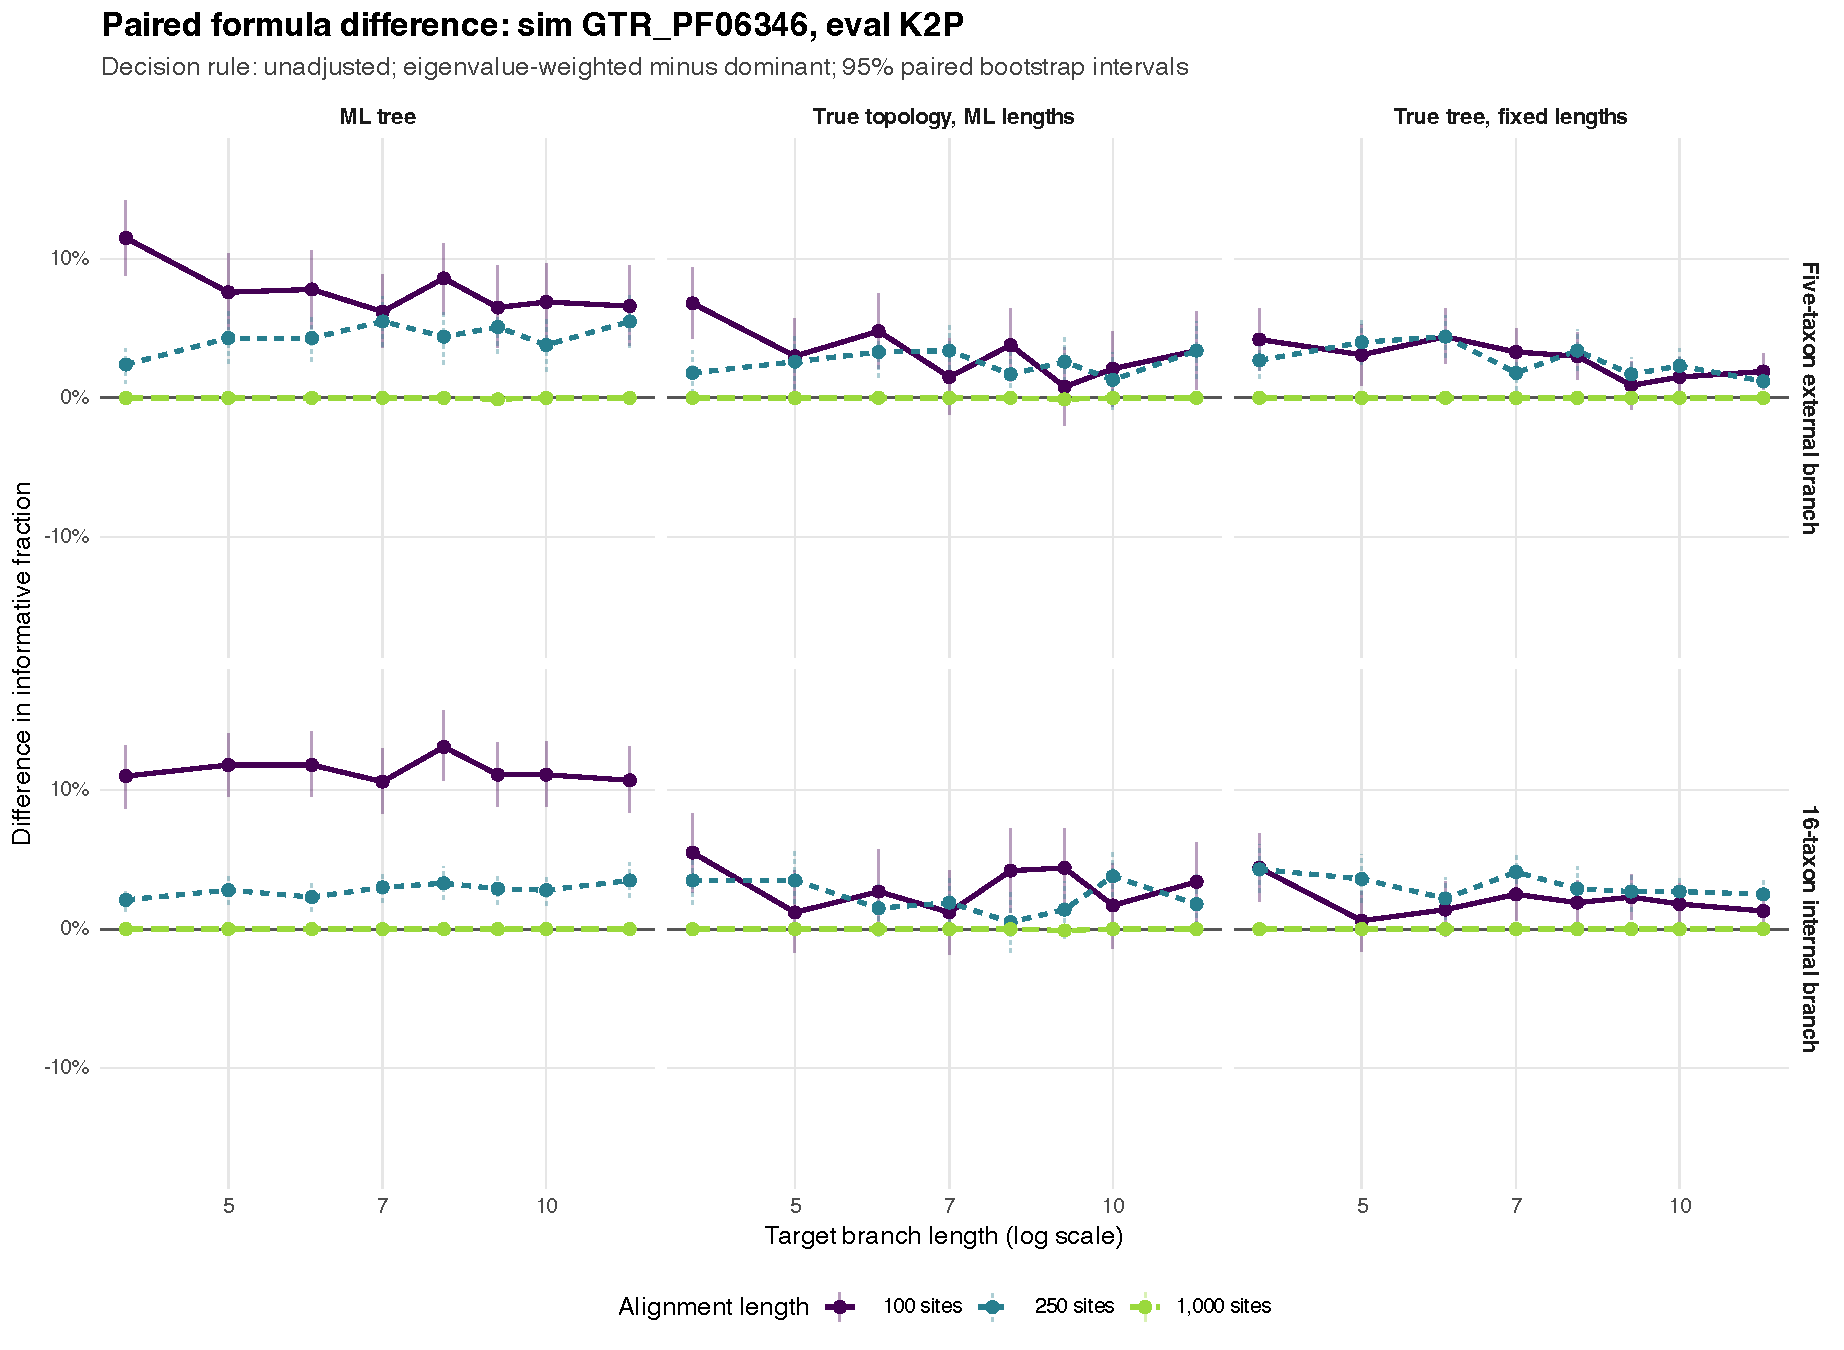
\includegraphics[width=0.32\textwidth]{figures/publication-suite/figure_gtr_misspec_K2P_paired_difference_2d.pdf}
  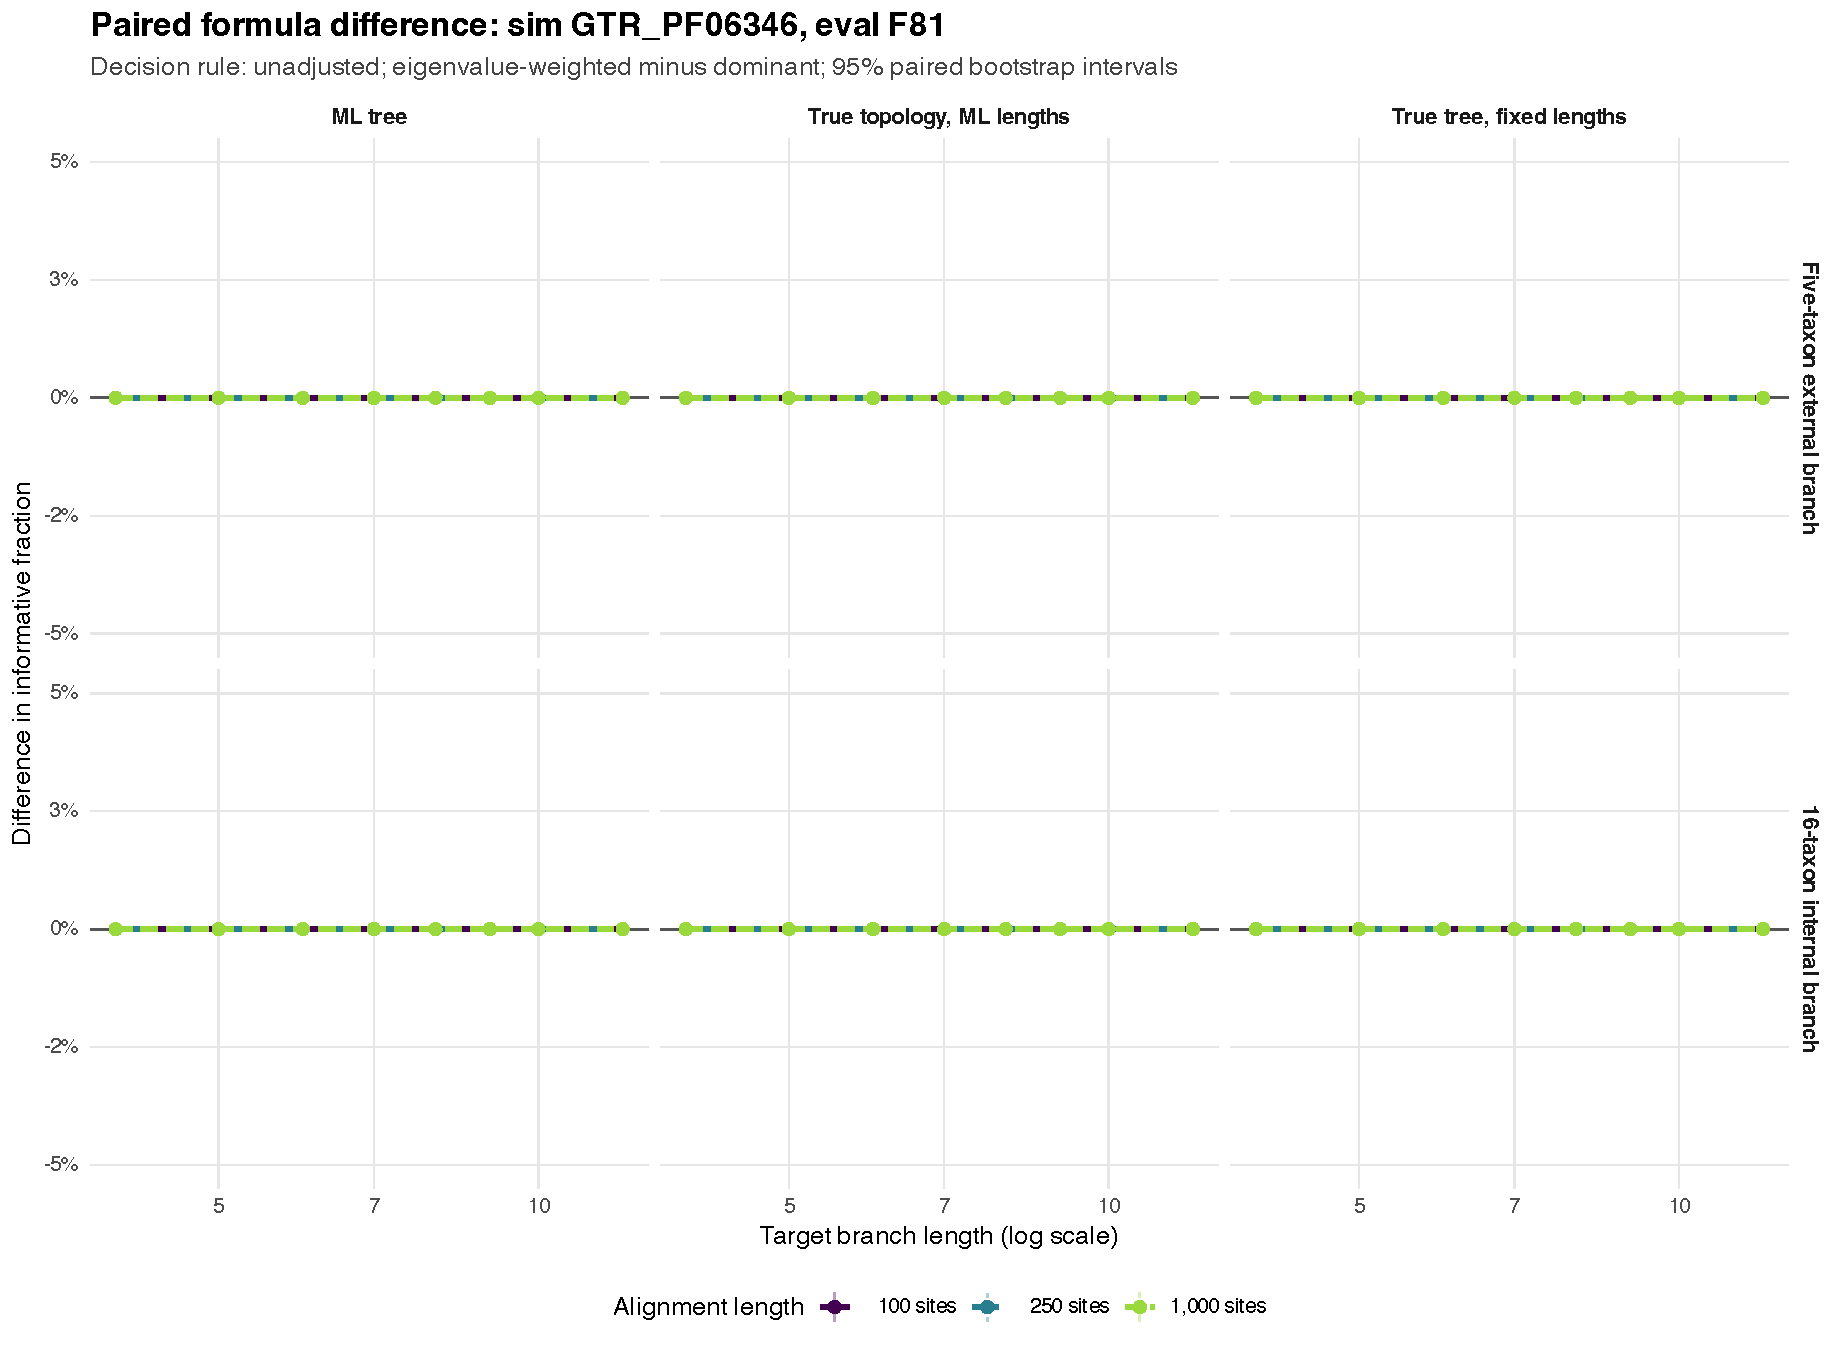
\includegraphics[width=0.32\textwidth]{figures/publication-suite/figure_gtr_misspec_F81_paired_difference_2d.pdf}
  \caption{\textbf{GTR model-misspecification comparisons.} Paired differences
  between the eigenvalue-weighted and dominant formulas when the same GTR+F
  simulations are evaluated by JC, K2P, and F81.}
  \makeatletter\cref@old@label{fig-gtr-misspec}\makeatother
\end{figure}

\begin{figure}[p]
  \centering
  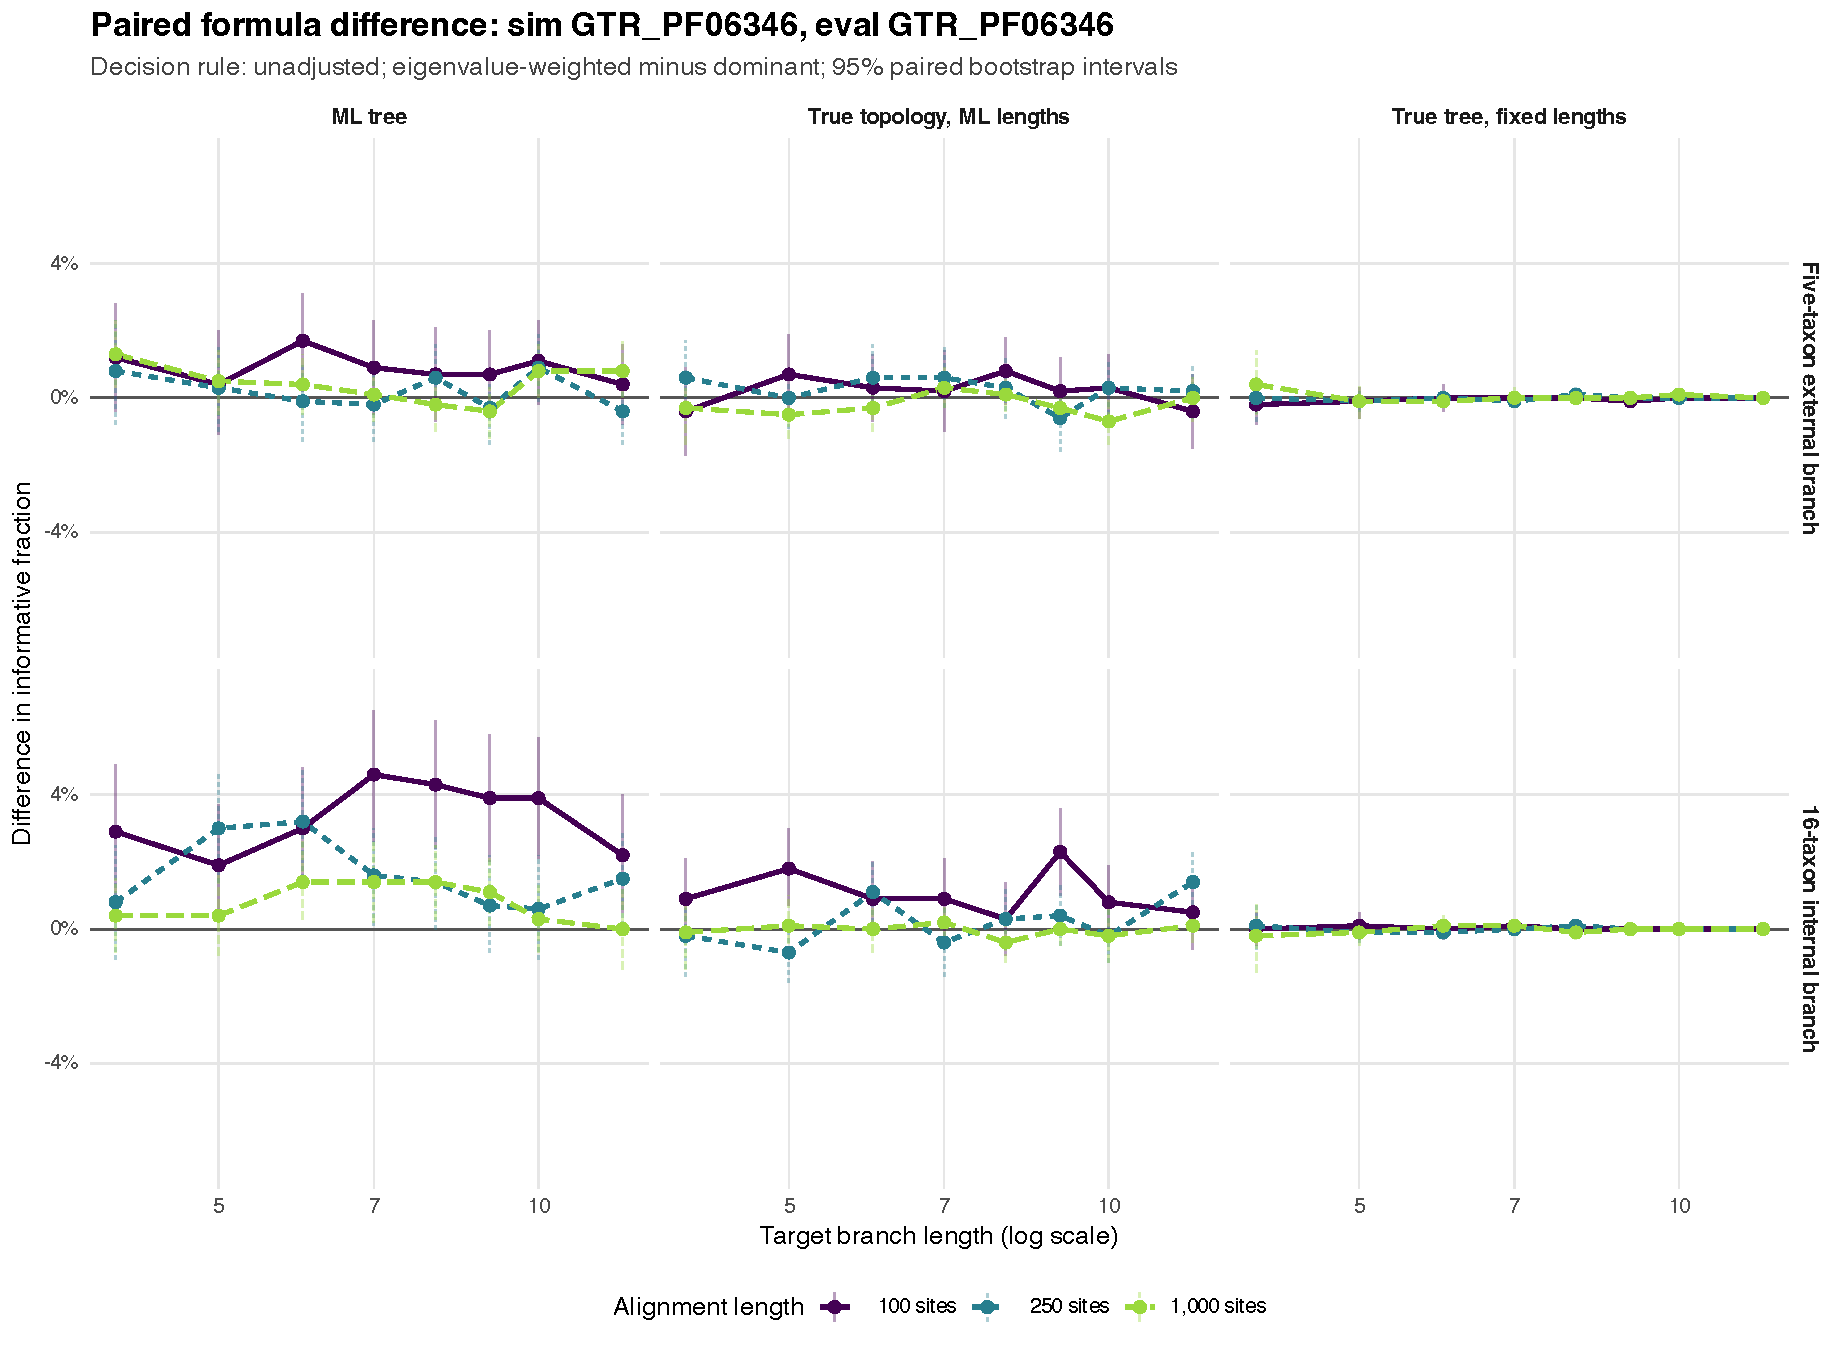
\includegraphics[width=0.98\textwidth]{figures/publication-suite/figure_gtr_matched_paired_difference_2d.pdf}
  \caption{\textbf{Matched GTR paired difference.} Difference in informative-call
  fraction between the eigenvalue-weighted and published dominant formulas on
  the corrected 1,000-replicate grid. Curves are stratified by tree and
  analysis scenario; line styles encode alignment length.}
  \makeatletter\cref@old@label{fig-gtr-matched-2d}\makeatother
\end{figure}

\begin{figure}[p]
  \centering
  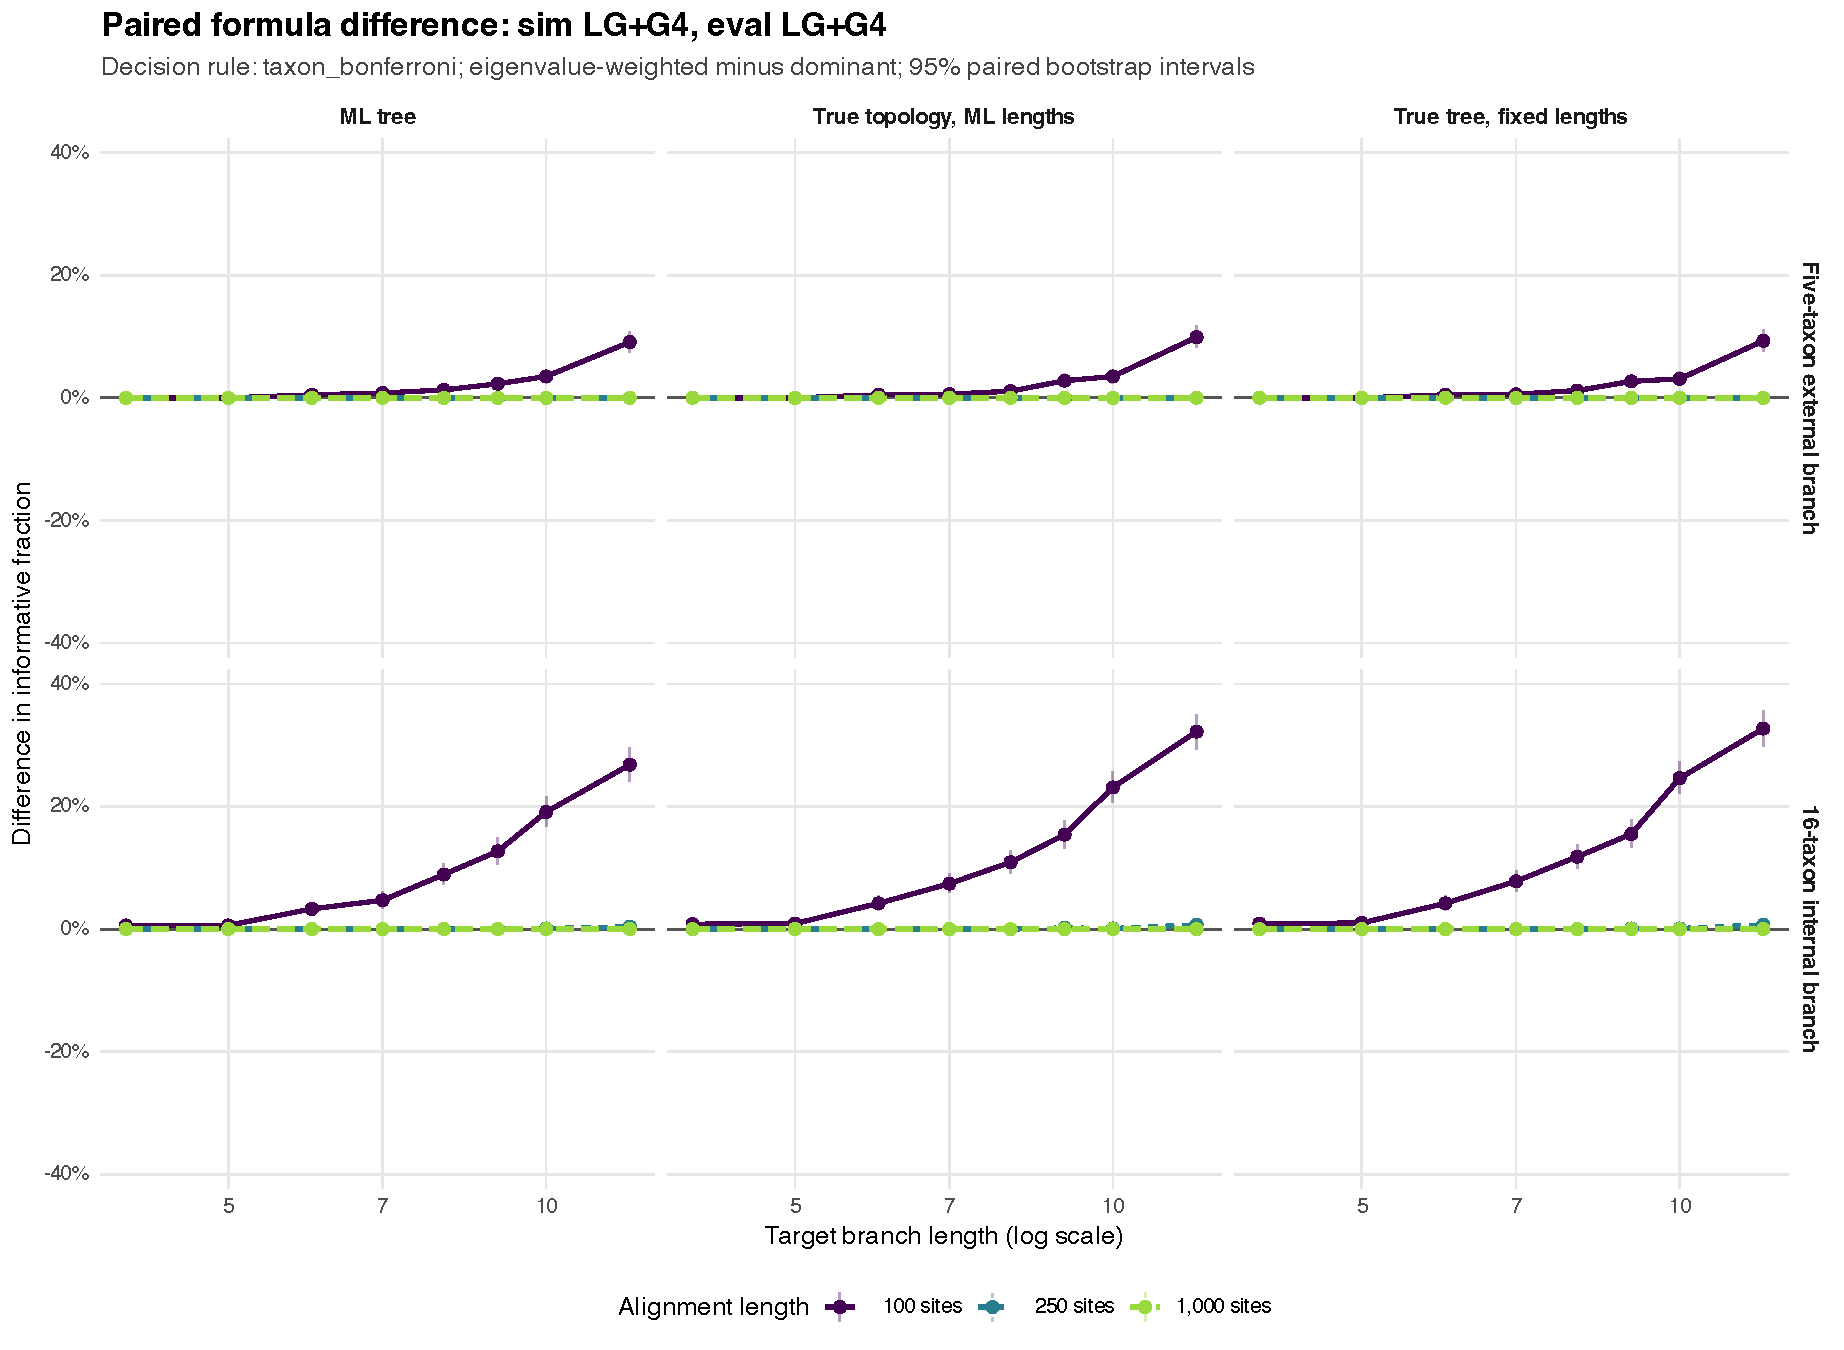
\includegraphics[width=0.49\textwidth]{figures/publication-suite/figure_protein_LG_G4_taxon_bonf_paired_difference_2d.pdf}
  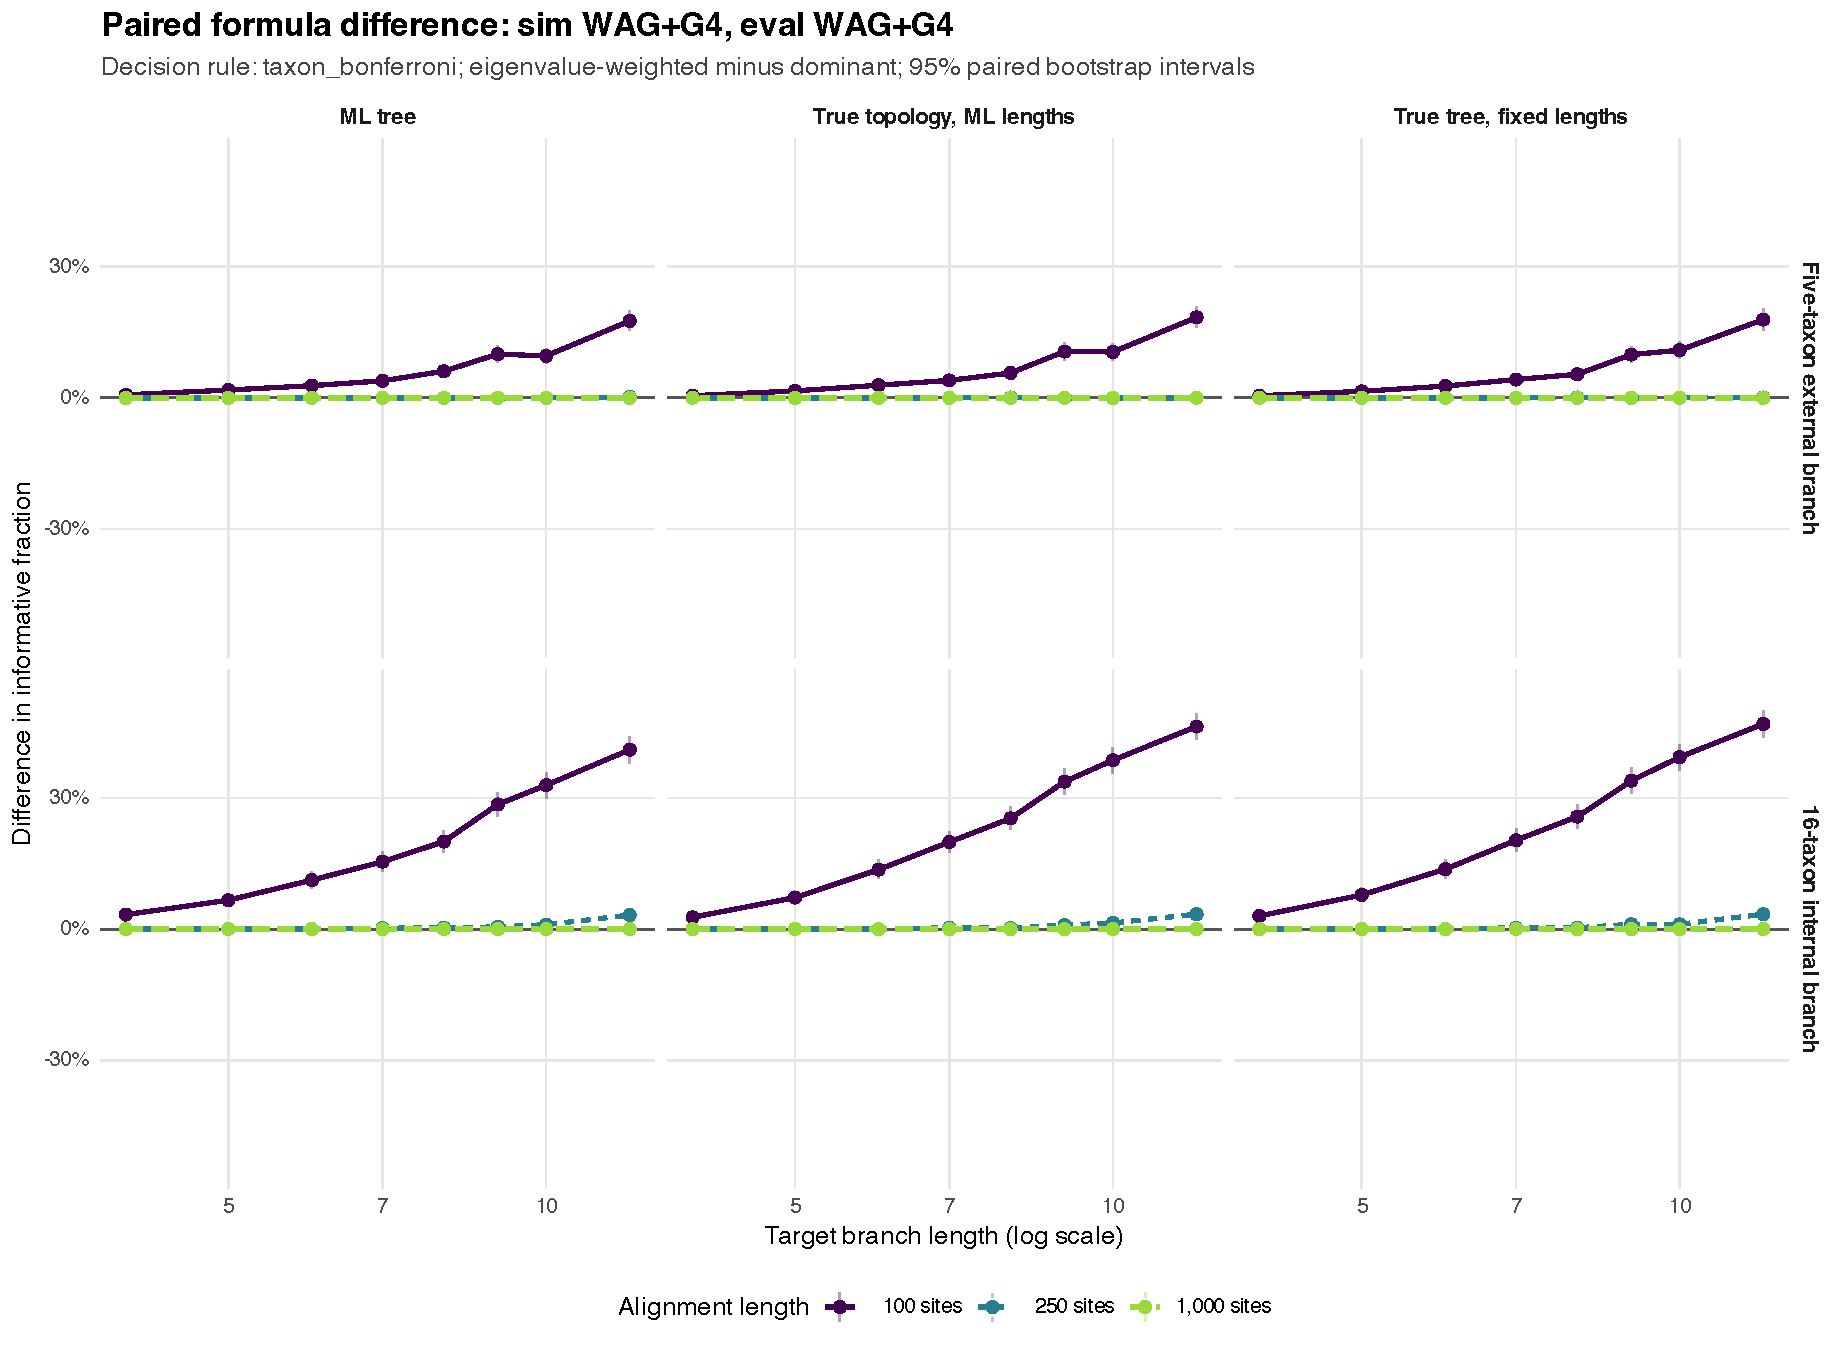
\includegraphics[width=0.49\textwidth]{figures/publication-suite/figure_protein_WAG_G4_taxon_bonf_paired_difference_2d.pdf}
  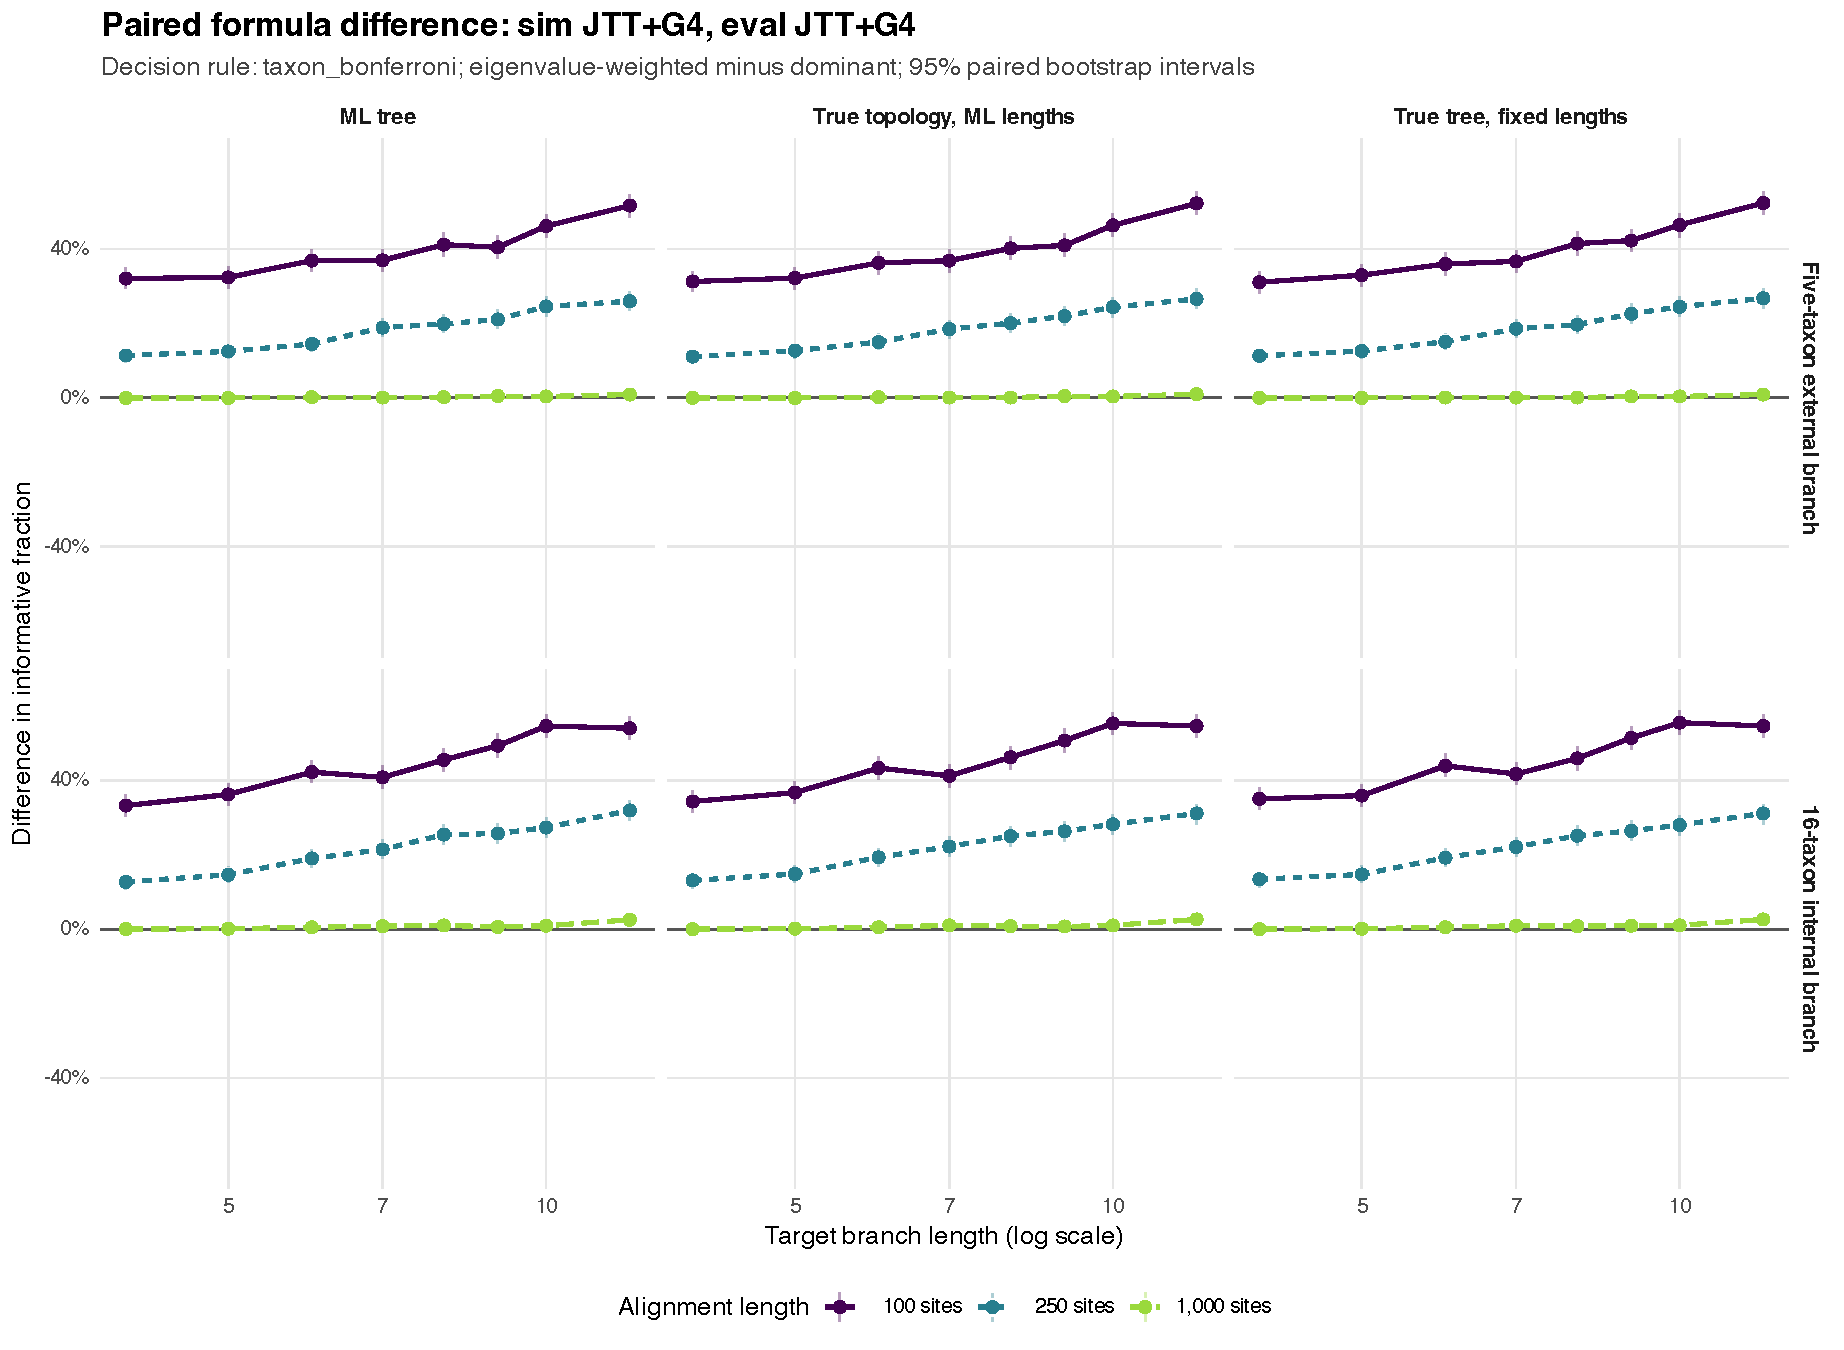
\includegraphics[width=0.49\textwidth]{figures/publication-suite/figure_protein_JTT_G4_taxon_bonf_paired_difference_2d.pdf}
  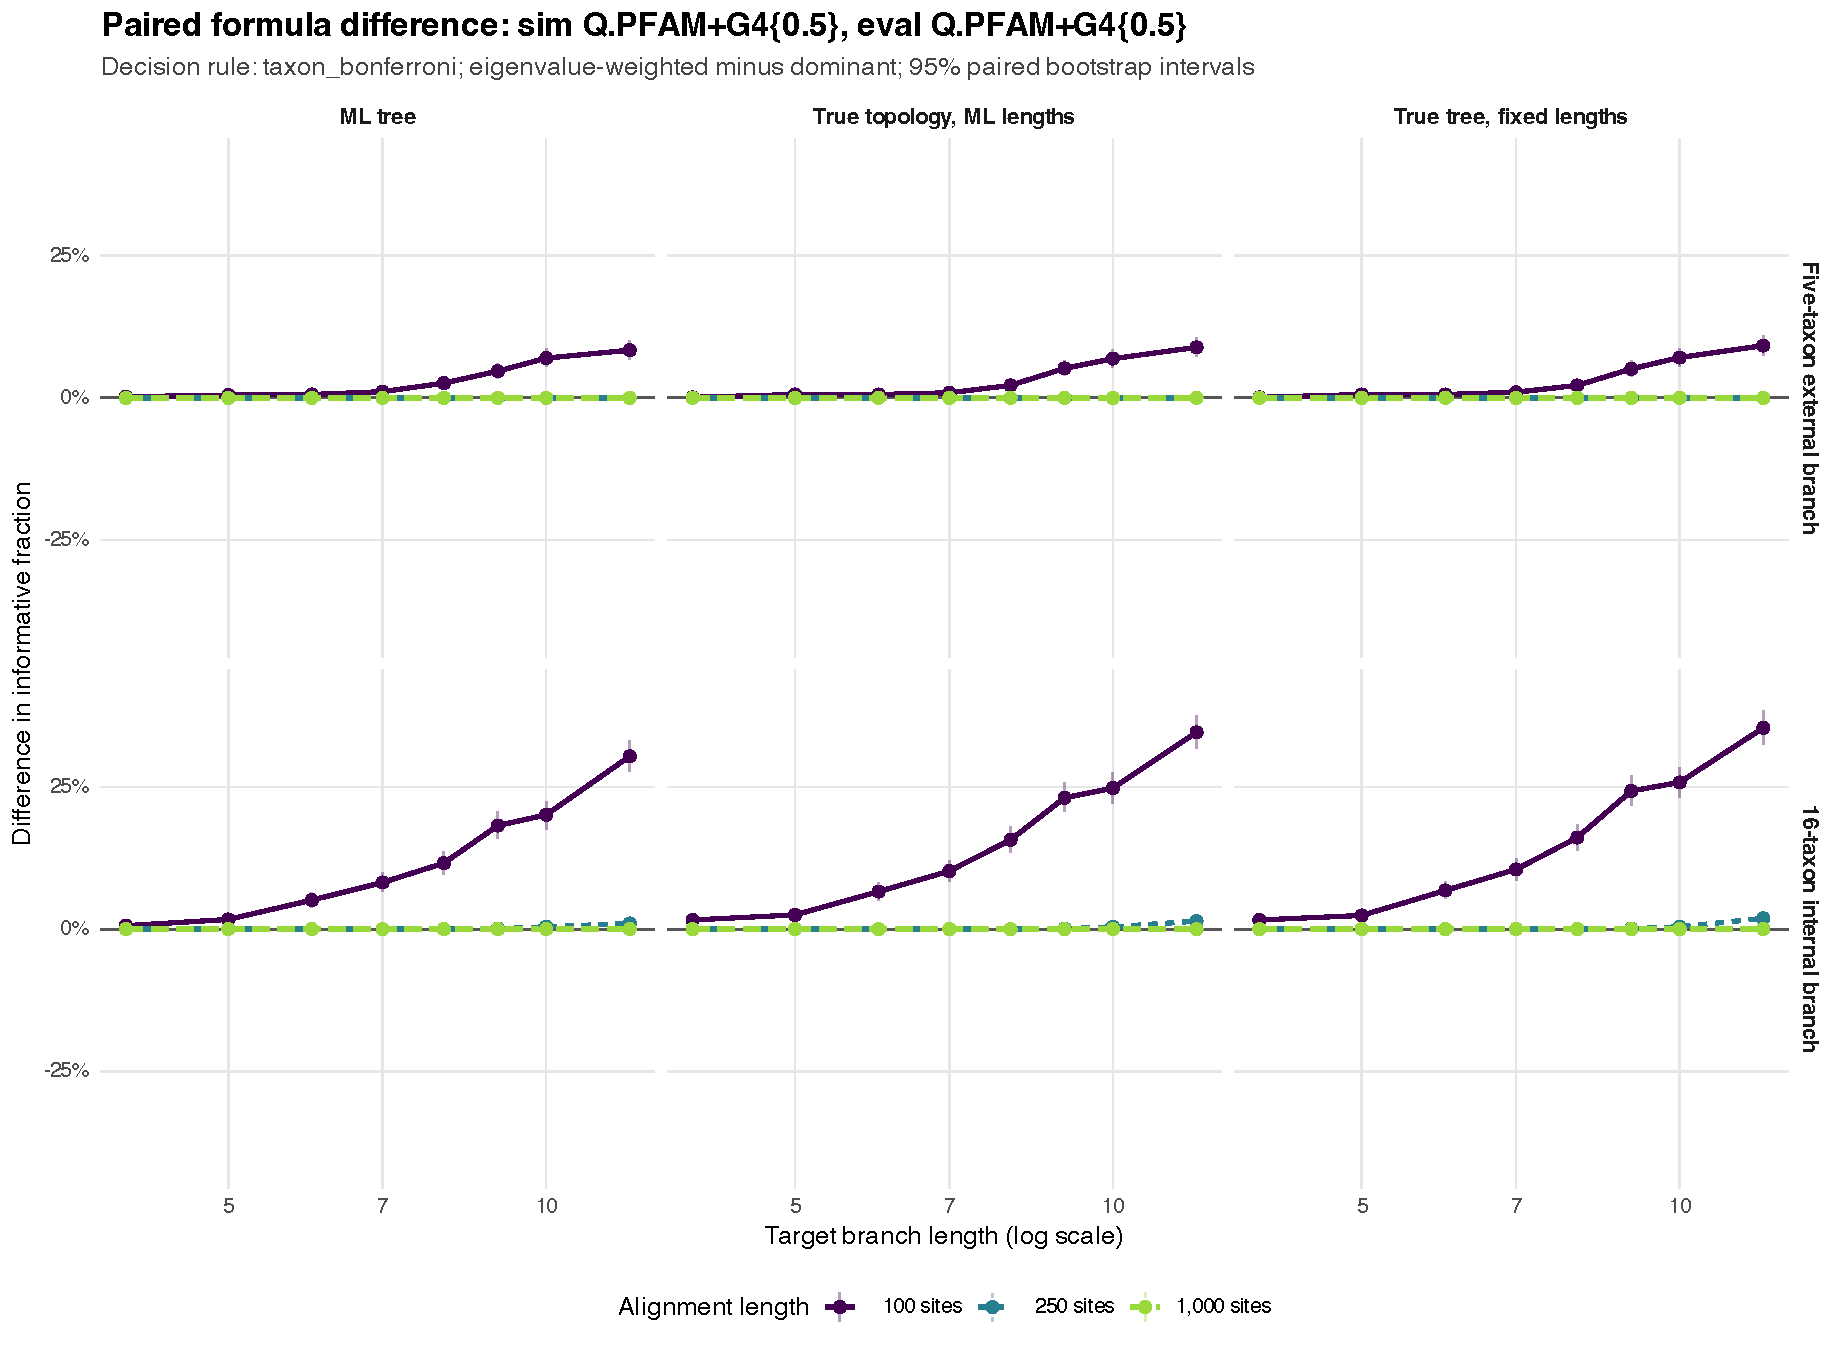
\includegraphics[width=0.49\textwidth]{figures/publication-suite/figure_protein_Q_PFAM_G4_taxon_bonf_paired_difference_2d.pdf}
  \caption{\textbf{Matched protein results under taxon Bonferroni.} Paired
  weighted-minus-dominant differences for fixed LG+G4, WAG+G4, JTT+G4 and
  Q.pfam+G4 models. Every panel uses the same 1,000 paired replicates per
  evaluated cell and reports bootstrap 95\% intervals.}
  \makeatletter\cref@old@label{fig-protein-bonferroni}\makeatother
\end{figure}

The FDR calibration suite is independent of the publication curves.  It uses
5,000 exact-null replicates (2,500 training and 2,500 held out) and 2,000
50:50 mixed-null replicates.  It reports unadjusted, taxon-Bonferroni, and
Benjamini--Yekutieli empirical FDR, power, held-out-null calibration, and
paired differences. In the GTR mixed-null design, power ranged from 0.929 to
0.989 across formulas, rules, tree cases, site counts and branch lengths,
whereas empirical FDR ranged from zero to 0.00386. Formula-paired power
differences were between \(-0.000071\) and 0.000571, and paired empirical-FDR
differences were between \(-0.000071\) and 0.000143. Thus the truth-labelled
experiment verifies high alternative detection and low false-discovery rates
for both formulas; the larger formula effects in the publication curves arise
at the saturation decision boundary rather than from global miscalibration.

Training-derived exact-null thresholds were evaluated on 2,500 independent
held-out nulls per cell. Across all 96 cells, held-out rejection ranged from
0.0108 to 0.0644. Unadjusted and Benjamini--Yekutieli GTR cells ranged from
0.0432 to 0.0596, while the discrete 16-taxon taxon-Bonferroni cells were
conservative because only complete adjusted-\(p\)-value tie blocks are
attainable. The calibration figures are generated independently in 2D and
vector 3D formats; the weighted GTR operating characteristics and held-out
calibration are shown in Fig.~\ref{fig-fdr-gtr}.

\begin{figure}[p]
  \centering
  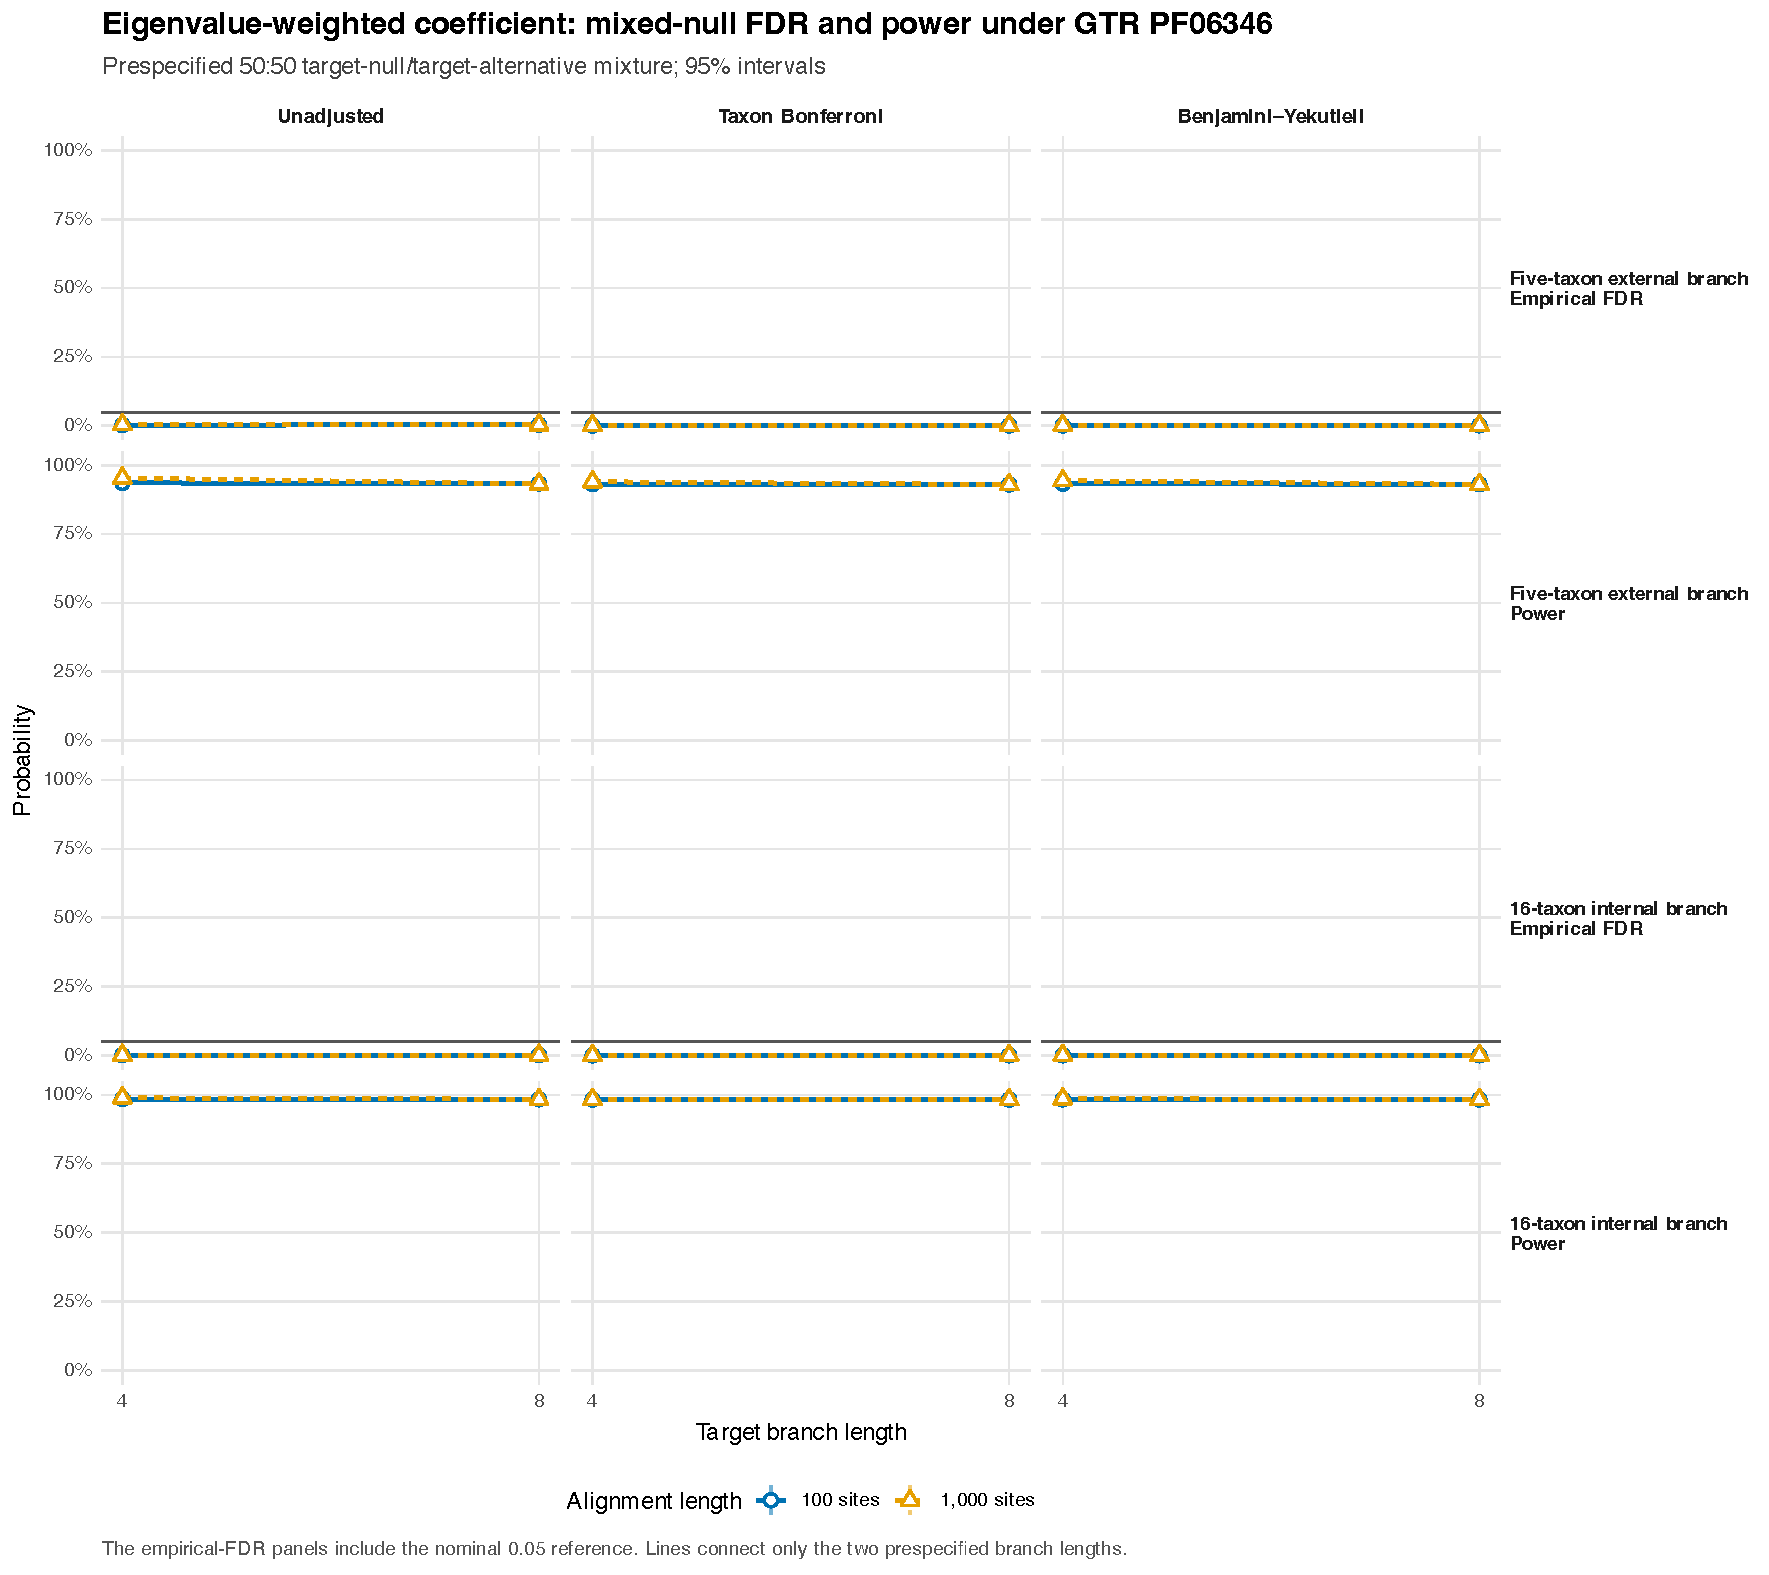
\includegraphics[width=0.48\textwidth]{figures/publication-suite/figure_fdr_weighted_power_2d_gtr.pdf}
  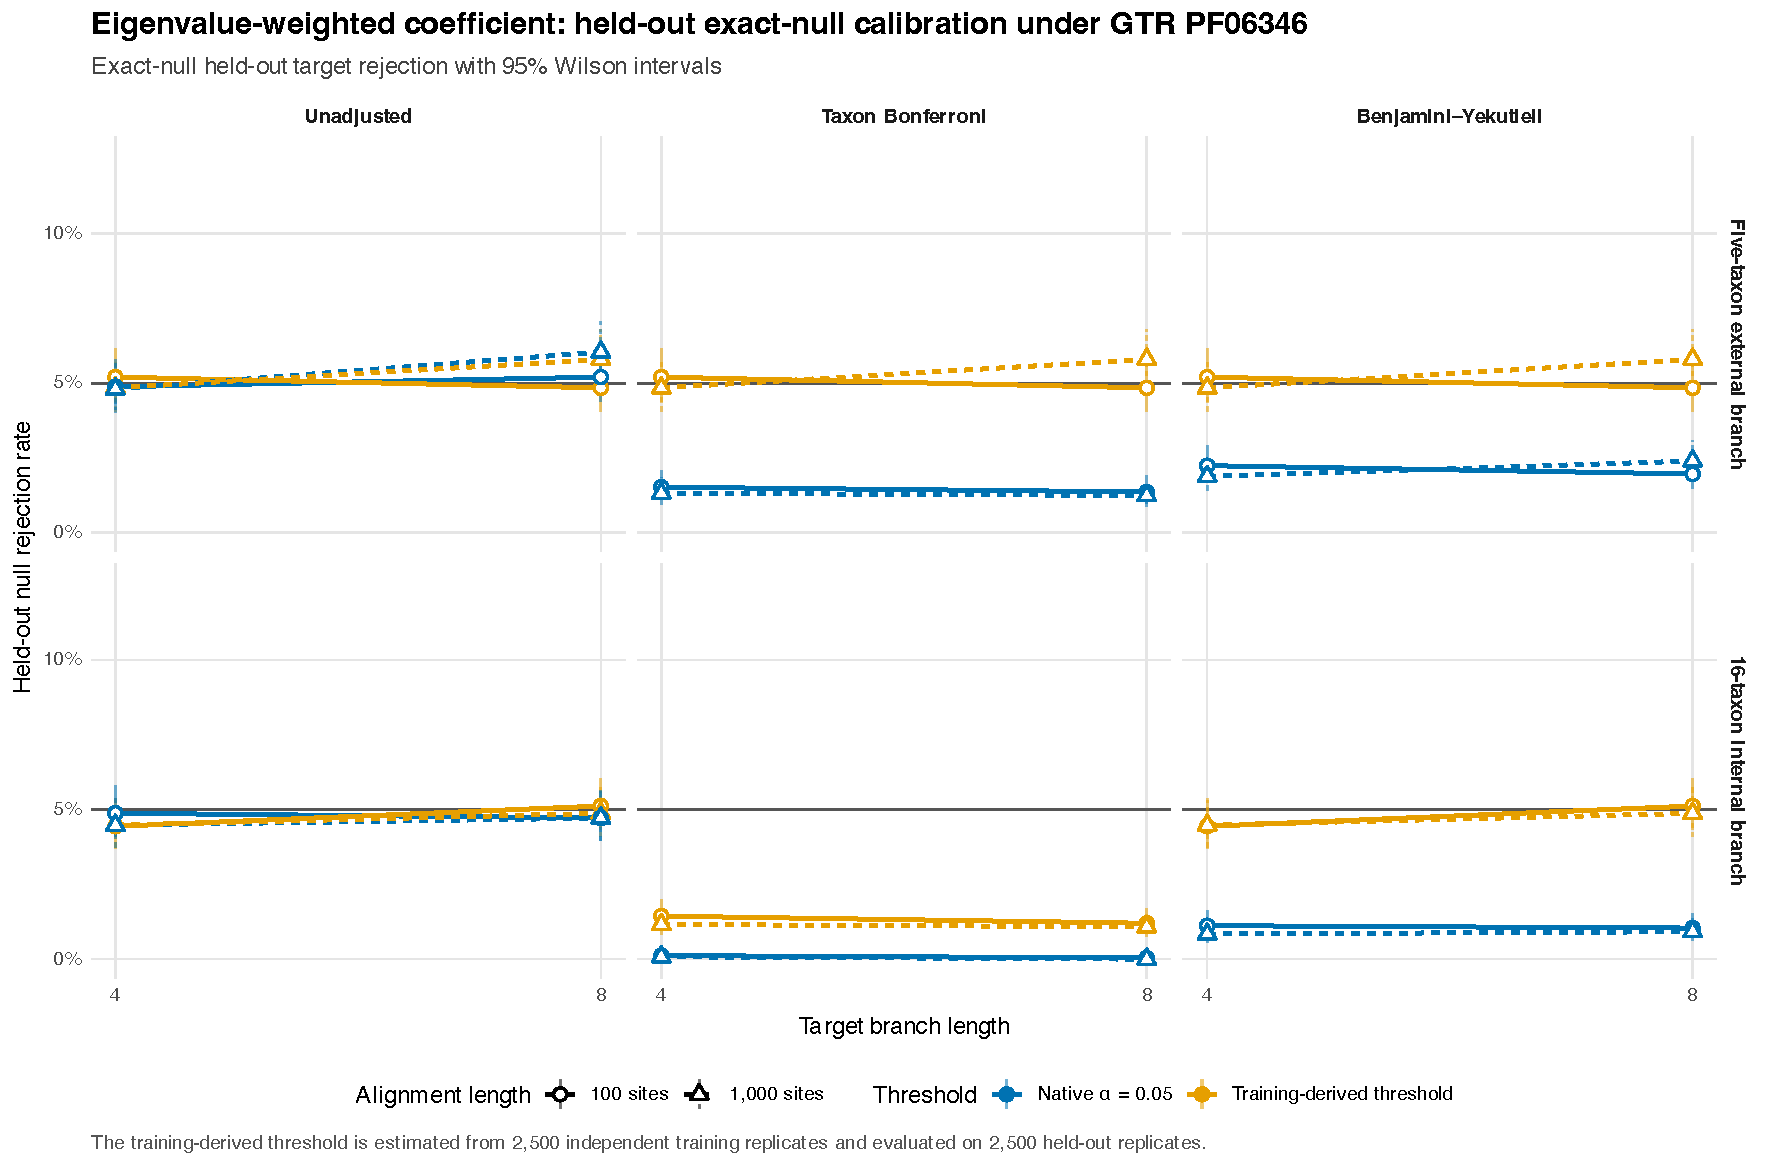
\includegraphics[width=0.48\textwidth]{figures/publication-suite/figure_fdr_weighted_null_calibration_2d_gtr.pdf}
  \caption{\textbf{Truth-labelled GTR calibration.} \textbf{Left,} empirical
  FDR and power of the eigenvalue-weighted formula in the prespecified 50:50
  mixed-null design. \textbf{Right,} native and training-derived exact-null
  rejection on 2,500 held-out replicates per cell. Columns show the
  unadjusted, taxon-Bonferroni and Benjamini--Yekutieli rules.}
  \makeatletter\cref@old@label{fig-fdr-gtr}\makeatother
\end{figure}
